\documentclass[12pt]{amsart}
\usepackage{float}
\newtheorem{theorem}{Theorem}
\usepackage{hyperref}

\usepackage[letterpaper, margin=1in]{geometry}
\usepackage{amssymb}
\usepackage[final]{graphicx}


\begin{document}

\title{Introduction to Network Problems and the Network Simplex Method}

\author{Stefano Fochesatto}

\date{\today}

\maketitle

\section{Introduction}
The network simplex method is a refined form of the simplex method which, as the name suggests is used for 
a special class of linear programming problems that are derived from networks. Network problems can come from 
several settings, such as optimizing road systems, telephone lines and personnel management.


%here is how to put in a figure:
%\begin{figure}
%\includegraphics[width=0.5\textwidth]{foo.png}  % put image "foo.png" in current directory
%\caption{CAPTION TEXT HERE}
%\end{figure}

\section{Terminology}  
A \emph{network} or \emph{graph} is defined by a set of vertices and a set of edges i.e we define a graph $G$ like so $G = (V, E)$
where $V$ is a set of vertices, and $E$ is a set of edges. \emph{Vertices} (also called nodes or points) 
are simply mathematical abstraction of the objects in our problems, in the context of road systems a vertex could represent 
an intersection, or a general location. An \emph{edge} (also called link or line) is simply an ordered pair of vertices, meant to describe the 
relationship between vertices, again in the context of road systems an edge might represent the street connecting two locations, or intersection.
An $\emph{arc}$ (or directed edge) define a relation between two vertices that is not symmetric, meaning if vertex $a$ is related to vertex $b$
it is not guaranteed that vertex $b$ is related to vertex $a$. In the context of road systems one could think of arcs as one-way streets.


A \emph{path} is a sequence of distinct arcs, connecting two vertices with no repeated vertices. We say that a graph is \emph{connected} if 
for every pair of vertices there exists a path connecting them. A \emph{cycle} is a path which begins and ends at the same vertex. A \emph{tree}
is a graph with no cycles. A \emph{subgraph} is a graph whose vertex and edge set is a subset of a larger graph, i.e. let $G = (V, E)$
and $A = (V', E')$ is a subgraph if $V'\subseteq V$ and $E'\subseteq E$. A \emph{spanning tree} is a subgraph which contains every vertex and is also a tree.  

\section{Types of Network Problems}
The main goal of every network problem is to move some entity, usually modeled by flow but can represent 
anything electricity, commodity, person or vehicle from one point to another in an underlying network as efficiently as possible. 
As we will see there are several different flavors of network problems such as \emph{shortest-path}, \emph{maximum-flow}, \emph{minimum-cut}, 
and \emph{assignment}. Each of these problems can be formulated as a special form of the more generalized \emph{Minimum Cost Network Flow Problem}.

\subsection{Minimum Cost Network Flow}
Suppose you have a directed graph (or network) where each vertex is assigned a value of flow and the weights assigned to 
the edges represent the cost of moving one unit of flow. Consider the example below, where $b$ is a vector of flow and $c$ is 
a vector of cost values. Assume flow at a vertex is 0 unless stated otherwise.  

\begin{figure}[H]
  \begin{center}
    \caption{Graph $G = (V, E)$ with flow $b$ and weights $c$}
    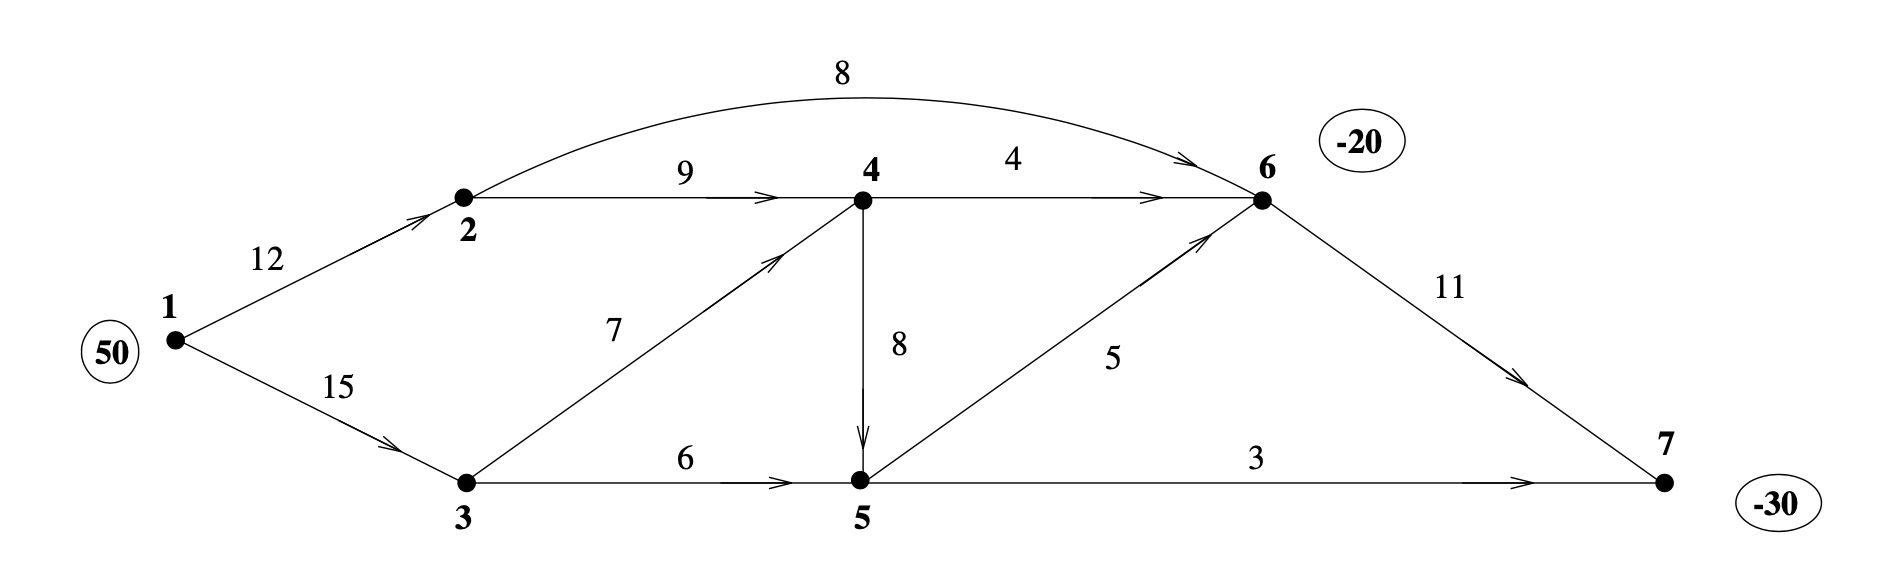
\includegraphics[width=.90\textwidth]{SampleNetwork.png}
  \end{center}
\end{figure}

If a vertex has positive flow we call it a source, and if vertex has negative flow we call it a sink. 
We define Supply, $S$ as 
\begin{equation*}
  S = \sum_{b_i > 0\in b}b_i,
\end{equation*}
and Demand, $D$ as
\begin{equation*}
  D = \sum_{b_i < 0 \in b}b_i.
\end{equation*}
We call a network balanced if $S - D = 0$, and an unbalanced network can be made balanced by adding an artificial vertex with flow $S - D$ by a directed edge with 
zero cost.\\


The goal of the minimum cost network flow problem is to satisfy the supply and demand of each vertex while minimizing the cost. Naturally the objective function will look 
like this, 
\begin{equation*}
    \mathop{\text{minimize: }}_{x}  z = c^Tx
\end{equation*}
where $x_{i,j} \in x$ represents the amount of flow through arc $(i, j)$, and we denote $c_{i, j}$ as the cost assigned to arc $(i, j)$. It's important to note that at the moment we are thinking of $x$ and $c$ as vectors, so this indexing is just for identifying 
the corresponding arc, not some location on a matrix. A feasible solution to this problem is an $x$ which satisfies the supply and demand of each vertex. 
With that context at each vertex $i$ our $x$ must satisfy, 
\begin{equation*}
  \sum_{j}x_{i, j} - \sum_{k}x_{k, i} = b_i.
\end{equation*} 
One can think of the first sum being flow out of vertex $i$ and the second sum being flow into vertex $i$. As an example consider vertex $1$ and $2$ in Figure 1, 
we get the following constraints
\begin{equation*}
  x_{1, 2} + x_{1,3} = 50,
\end{equation*}
\begin{equation*}
  x_{2, 4} + x_{2, 6} - x_{1, 2} = 0.
\end{equation*}
This is done for each vertex $i$, generating our constraint matrix $A$ which will be size (\# of vertices)$ \times $(\# of edges). Usually there will be some added constraints $L$ and $U$ on the amount of flow that can go through each edge, so most problems will be of the form, 
\begin{align*}
    \mathop{\text{minimize: }}_{x}  z &= c^Tx\\
  \text{subject to: }Ax &= b\\
  L \leq&x\leq U
\end{align*}



\subsection{Maximum Flow}
Suppose you have a directed graph with $m$ vertices but in this case, we only consider two special vertices, $1$ and $m$ where $1$ is 
the source and $m$ is the sink. The weights assigned to each arc represent the maximum capacity of flow that can move between vertices. \\


The goal of a maximum flow network problem is to maximize the amount of flow through the source and the sink without overwhelming the capacity of 
the network. So a solution to the maximum flow network problem determines the maximal amount of flow that can be moved from source to sink, as well as the 
routing of that flow across the network. 

To formulate the problem as a linear program, as before let $x_{i, j} \in x$ represent the amount of flow through arc $(i, j)$, let $u_{i, j}$
represent the capacity of arc $(i, j)$. Let $f$ be the amount of flow in the network. Then our problem can be written in the following form, 
\begin{align*}
    \mathop{\text{maximize: }}_{x, f} &z = f\\
    \text{subject to: } &\sum_{j}x_{1, j} - \sum_{k}x_{k, 1} = f,\\
    &\sum_{j}x_{i, j} - \sum_{k}x_{k, i} = 0, \quad i = 2, \dots, m - 1\\
    &\sum_{j}x_{m, j} - \sum_{k}x_{k, m} = -f,\\
    &0 \leq x_{i, j} \leq u_{i, j}.
\end{align*}
Naturally since we wish to find the maximum flow $f$, between vertices $1$ and $m$ through the network, vertex $1$ will have a surplus of flow $f$ and 
$m$ will have a demand of flow $f$. Since all the flow is moving from $1$ to $m$ all vertices in between must be balanced, hence the 0 on the right hand side
of the middle equality constraints. Finally the inequality constraints come from our desire to not overwhelm the capacity of the network. 

We can convert the maximum flow problem into a minimum cost network flow problem. Suppose we add an an artificial arc $(1, m)$ with unlimited 
capacity $u_{m, 1}$. Then the problem can reformulated by, 
\begin{align*}
    \mathop{\text{minimize: }}_{x} &z = -x_{m, 1}\\
    \text{subject to: } &\sum_{j}x_{i, j} - \sum_{k}x_{k, i} = 0, \quad i = 1, \dots, m\\
    &0 \leq x_{i, j} \leq u_{i, j}
\end{align*}
To see this let $x_{m,1} = f$ and by substitution the constraints are equivalent. Since minimum cost network flow is a minimization problem we multiply
the cost function by $-1$, hence $z = -x_{m, 1}$. To see this in the previously stated matrix vector form of the minimum cost network flow problem, let 
$b = 0$, let $c$ be a one hot vector with $c_{m,1} = -1$, let $L = 0$ and, let $U = u$ a vector of arc capacities. 


\section{Network Simplex}
\subsection{Feasibility}
The crux of the network simplex method lies in two key ideas and we will explore them in the context of a 
minimum cost network flow problem with only positivity constraints. Let $G = (V, E)$ be a network on $m$ vertices and recall the minimum cost network flow problem, 
\begin{align*}
    \mathop{\text{minimize: }}_{x}  z &= c^Tx\\
  \text{subject to: }Ax &= b\\
  x \geq& 0
\end{align*}
By our definition of $x_{i, j} \in x$ as the flow between arc $(i, j)$ we know that the columns of our constraint matrix $A$ represent 
the arcs in our network. Since we constructed each row of our matrix $A$ by examining the flow across a single vertex, we know that each row represents a vertex. So in the column view, a column representing arc $(i, j)$ will have a $1$ in the row representing vertex $i$ and a $-1$ in the row representing 
vertex $j$. In the row view, a row representing vertex $i$ will have a $1$ in every column representing arc $(i, k)$, and a $-1$ in every row representing arc $(k, i)$ where 
$k \in V$. The first big idea comes as the following theorem.
\begin{theorem} Let $B$ be a submatrix of the constraint matrix $A$ whose columns represent the edges of a spanning tree.
    Then $B$ is a full column rank matrix with dimension $m \times (m - 1)$, and it can be rearranged so that the diagonal entries are $\pm 1$. 
\end{theorem}

There is a sense that this result feels intuitive, clearly a spanning tree on a connected graph with $m$ vertices must have $m - 1$ arcs. Showing that 
$B$ can be rearranged follows by a proof by induction (you can find it on p.285 of Griva). 

% Maybe write it out

Recall that a basic solution $x$ to a general LP problem has non-zero entries, whose corresponding columns in the constraint matrix $A$ are linearly independent
and $x$ satisfies the equality constraints. We define a \emph{spanning tree solution} $x$, as a solution to the system $Ax = b$ where the non-zero entries of $x$
correspond to columns of $A$ which represent a spanning tree. A \emph{feasible spanning tree solution} is simply a spanning tree solution which also satisfies the 
positivity constraints, $x \geq 0$. The next big idea uses the previous theorem and definitions about spanning trees and connects them to LP, 
  
\begin{theorem} A flow $x$ is a basic feasible solution for the network flow constraints $Ax = b$ and $ x \geq 0$ if and only if it is a feasible spanning tree solution.  
\end{theorem}
The backwards direction follows directly from the previous Theorem 1 and the definition of feasible spanning tree solution. The forwards direction proceeds by contradiction supposing 
$x$ is a basic feasible solution and not a feasible spanning tree solution. If 
$x$ is not a spanning tree then it must have a cycle. Choose a vertex $i$ in the cycle, it must have arcs $(i, j)$ and $(k, i)$ for some $k$ and $j$ in the cycle.
The flow across an arc $(i, j)$ in the cycle may be increased by some $\epsilon \geq 0$, and in order to stay feasible we must decrease the flow across the arc $(k, i)$. 
So we have a new flow $x_\epsilon$, we can construct another flow $x_{-\epsilon}$ by subtracting $\epsilon$ from the flow across $(i, j)$ and adding $\epsilon$ to $(k, i)$.
%% Add image. 
Finally note that, 
\begin{equation*}
    x = \frac{1}{2}x_{\epsilon} + \frac{1}{2}x_{-\epsilon}.
\end{equation*}
Therefore $x$ is not an extreme point in the feasible set and by the Fundamental Theorem of Linear Programming $x$ is not a basic feasible solution. 

\subsection{Network Simplex} 
The network simplex method proceeds in a similar fashion, to the general simplex method with a few improvements on how we 
compute each step. First note that we must initialize the algorithm, just like the regular simplex method with basic feasible solution. One could 
conceivably implement the first step problem to find a BFS. Like in the regular simplex method we'll need to form our Basis and Null matrices $B$ and $N$
respectively. As we have shown in the previous section our $B$ matrix will be full column rank with dimension $m \times (m - 1)$ and the $N$ matrix 
will have columns which represent all the arcs that didn't show up in our feasible spanning tree. Recall that the first step in the simplex method is to compute
simplex multipliers $y$ by solving the system, 
\begin{equation*}
    B^Ty = c.
\end{equation*}
Here is where we can take advantage of Theorem 1 to make solving this system faster. Note that $B^T$ is a full row 
rank $(m - 1) \times m$ matrix, so we are guaranteed when solving $B^Ty = c$ to have a free variable. Since $B^T$ is 
a matrix whose rows now represent edges, solving this system by back substitution produces the following expression, 
\begin{equation*}
    y_i - y_j = c_{i, j}
\end{equation*} 
where $y_i$ and $y_j$ are the simplex multipliers associated with vertices $i$ and $j$ and $c_{i, j}$ is the cost associated to 
arc $(i, j)$. This means that we can compute the simplex multipliers by selecting a vertex $i$ to correspond to our free simplex multiplier, so we will let $y_i = 0$ 
and we compute the rest $y_j$ by traversing the feasible spanning tree computing $y_j = y_i - c_{i,j}$ along the way.  


Computing the reduced costs is no different from the regular simplex method, we use $\hat{c}_{i, j} = c_{i, j} - N^Ty$. Again choosing which arc becomes the new entering arc is no different, 
simply find the minimum $\hat{c}_{i, j}$ and consider the corresponding arc $x_{i, j}$ in the columns of $N$. Then we check our optimality conditions just as before, are $\hat{c}_{i, j} \geq 0$. 


To choose our leaving arc, we will be taking advantage of Theorem 2 and a small result about spanning trees. Taking our entering arc $x_{i, j}$ and adding it into our spanning tree graph, it is 
guaranteed that this will produce a single undirected cycle that includes the arc $x_{i, j}$. By Theorem 2 adding this arc $x_ {i, j}$ into our solution makes us no longer basic. 
In order to stay feasible and basic, we must remove an arc from the cycle to get back to a spanning tree, and increase the flow through $x_{i, j}$ and appropriate amount to satisfy our equality constraints. Here's the trick, 
locate the edges in the cycle which point in the opposite direction as $x_{i, j}$, we'll call them negative edges. Let $m$ be the minimum flow through those negative edges. Set $x_{i, j} = m$ and 
subtract $m$ from all negative $x_{l, k}$ in the cycle. This operation maintains basic feasibility since the minimum flow $x_{l, k}$ arc gets removed from our solution becoming our exiting variable and our 
entering variable in increased enough to satisfy the equality constraints. Also note that if there is no minimum flow $x_{l, k}$, and $x_{i, j}$ can be increased arbitrarily than
the problem is unbounded, just like in the regular simplex method. 

The steps are then repeated with the new feasible spanning tree solution until we achieve the optimality conditions. 


\section{Implementation} Consider the example defined in Figure 2, of a positively constrained minimum cost network flow problem.
\begin{figure}
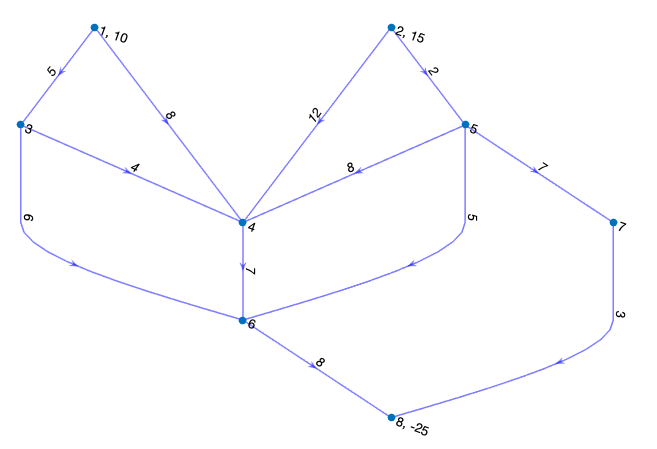
\includegraphics[width=.80\textwidth]{untitled.png}  % put image "foo.png" in current directory
\caption{Our given network which defines $A$ and $b$, by network structure and flow. }
\end{figure}

\begin{figure}
    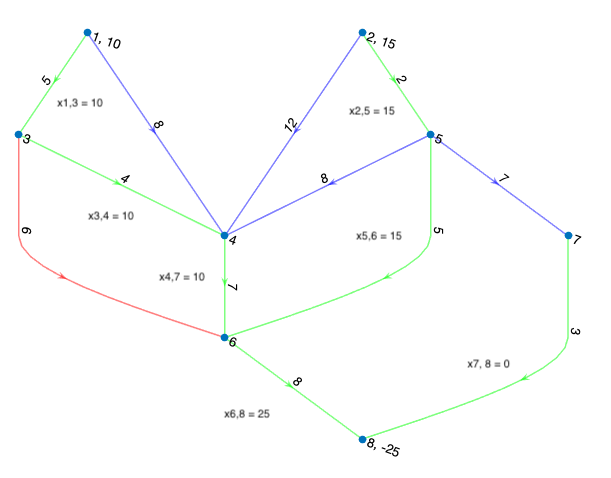
\includegraphics[width=.80\textwidth]{step1.png}  % put image "foo.png" in current directory
    \caption{Initial feasible spanning tree shown in green. Red is the entering arc for this first iteration.}
    \end{figure}
    Our initial feasible spanning tree solution outlined in green in Figure 3. Again the equations for computing the simplex multipliers allows us to simply set 
    the multiplier associated with vertex 1 to zero, so we get $y_1 = 0$. To solve the next multiplier we traverse the green spanning tree to vertex 3 and in doing so we solve 
    for $y_3$ with $y_3 = y_2 - c_{1,3} = 0-5 = -5$. Solving the next multiplier we get $y_4 = y_3 - c_{3, 4} = -5 - 4 = -9$ and so on. 

    Once we have the simplex multipliers together we can solve for the reduced costs of the nonbasic arcs. Doing so we can check our optimality conditions, and in this 
    case there exists negative reduced costs, so we continue. You'll find that the reduced cost for $x_{3, 6}$ (marked in red in Figure 3) is the lowest among the negative reduced costs and therefore becomes our 
    entering arc. 

    To solve for our exiting arc consider the cycle formed by vertices $\{3, 4, 6\}$. Note that $x_{3, 6}$ is pointing in the counter clockwise direction, and therefore we designate 
    arcs $x_{3, 4}$ and $x_{4, 6}$ as negative. Note that the minimum flow across the negative arcs is equal so when we subtract that flow from $x_{3, 4}$ and $x_{4, 6}$ and 
    add it to $x_{3, 6}$ both $x_{3, 4}$ and $x_{4, 6}$ will be zero and we will get to choose which of the two arcs becomes our exiting arc. 
    Choosing $x_{3, 4}$ to be the exiting arc and setting $x_{3, 6} = 10$ we arrive at the next feasible spanning tree solution. Figure 4 shows the final iteration of this problem, the working out is 
    left as an exercise to the reader.   
    \begin{figure}
        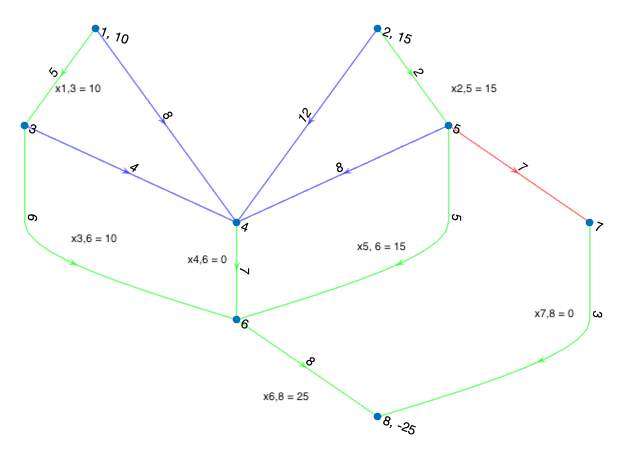
\includegraphics[width=.80\textwidth]{step2.png}  % put image "foo.png" in current directory
        \caption{In green is the resultant spanning tree from the first iteration. In red is the next entering arc for the second iteration.}
        \end{figure}

    You'll find code and an example, for running this method on positively constrained minimum cost flow network problems at the end of this paper. 


\section{Analysis and Conclusion}  
        Through some careful analysis of our constraint matrix $A$ and some elementary graph theory on the subject of spanning trees and cycles we were able 
        to reduce the FLOPs of the general simplex method significantly. In the general simplex method as we have studied it there are 
        three linear systems that have to be solved, namely $Bx_b = b$ for the basic variables of the current iterate, $B^Ty = c_b$ for the simplex multipliers, 
        and $B\hat{A_t} = A_t$ to perform the ratio test and find the exiting variable. Compared to the network simplex method, $Bx_b = b$ and $B\hat{A_t} = A_t$ are
        replaced by the cycle procedure that find us the exiting arc, and solves for the value of the entering basic arc. The $B^Ty = c_b$ computation is replaced by our 
        traversal of the feasible spanning tree solution, solving each simplex multiplier as we hop from vertex to vertex. 
    
        As you will see in the supplied code, what we trade in for efficiency we often need to make up for with clever data structures. You'll see that 
        there is a lot of index management across different representations of the network, in the form of adjacency and incidence matrices. Representing 
        the network with only these matrices makes these operations in the network simplex method cumbersome.  
        

\begin{thebibliography}{2}  % "2" because there are two references use  \cite{einstein}
\bibitem{grivanashsofer}
I.~Griva, S.~Nash, \& A.~Sofer (2009).
\textit{Linear and Nonlinear Optimization},
2nd ed., SIAM Press.
\end{thebibliography}




\newpage
You can find the code for this project on my \href{https://github.com/StefanoFochesatto/NetworkSimplex}{github page}.
\bigskip
\hrule
\begin{verbatim}
    function [graphHist ,bf , xf] = NetworkSimplex(s, e, c, b, x0, maxiter)
    % This implementation of network simplex solves the 
    % basic minimum cost network flow problem with only positivity constraints. 
    % We take in a directed arc set (s, e) where the arc starts at a vertex from 
    % s and ends at the corresponding vertex in e.
    % We also take in the and the associated cost of each vertex c. Finally we take in 
    % x0, an initial basic feasible solution and a vector b, a logical vector
    % for identifying the arcs of the feasible spanning tree. 
    % Input case for the example is commented at the bottom
    
    % First we need to form the correct incidence matrix A for our problem.
    G = digraph(s, e, c);
    A = -1*(incidence(G));
    [m, n] = size(A);

    % Set inital BFS
    x = x0;
    
    % Pull column indices for B and N matrix
    nullIndex = find(~b); 
    baseIndex = find(b);
    graphHist = {'Basic Spanning Tree', 'Proposed Flow'};
    
    
    
        for i = 1:maxiter
            % Compute the simplex multipliers
            y = NetworkSimpMulti(A, b, c, m);
    
            % Compute reduced costs
            cHat = reducedCosts(A, b, c, y);
    
    
            % Optimiality Check (moved this into here so I can update the graphHist). 
            if cHat >= 0
                xf = x;
                bf = b;
                break 
            end
    
    
            % This section of code runs through how the exit variable is chosen
            % First we select the arc which corresponds to the smallest reduced
            % cost and add it to our spanning tree. This must produce a unique
            % cycle. Set the direction (clockwise or counterclockwise about the cycle) 
            % of this new arc (our entering variable) to positive and let arcs
            % in the other direction in the cycle be negative. If we reduce the
            % negative arcs in the cycle by one unit of flow, to continue 
            % being a solution we need to increase the flow across the 
            % entering arc. 
            % To stay feasible we
            % continue this process until a negative arc has zero flow, and
            % therefore becomes the exiting variable. Finally we update the
            % basic and null indices to reflect our new iteration. 

            % enterIndex is index of edge in N
            [mincost, enterIndex] = min(cHat); 
            % Using nullIndex to pull index of edge from A
            enterArc = nullIndex(enterIndex);
    
            % Generating Digraph for proposed flow
            proposedFlow = 
                digraph(s([baseIndex, enterArc]),e([baseIndex, enterArc]), 
                    c(s([baseIndex, enterArc])));
       
            % Updating Hist
            graphHist(i,:) = 
                {digraph(s(baseIndex),e(baseIndex), 
                    c(s(baseIndex))), proposedFlow};
            
        
    
            % Pulling enter and exit vertex, for direction purposes
            startVertex = find(~(A(:, enterArc) - 1));
            endVertex = find(~(A(:, enterArc) + 1));
    
          
    
            % Find cycle in proposedFlow
            [targetCycle,targetCycleEdges] = 
                allcycles(graph(proposedFlow.adjacency + proposedFlow.adjacency'));
          
            % Checking that cycle is found
            if length(targetCycle)~= 1
                error('cycle not found or solution/ iteration was not BF')
            end
            
            % Pulling -1* cycle incidence matrix. 
            Cycle = -1*proposedFlow.incidence;
            Cycle = Cycle(:, targetCycleEdges{1});
    
            % Pull arc index from full incidence matrix A
            % I have to do this whole thing because the Cycle()
            % reorders the columns. 
            arcIndex = [];
            for j = 1:length(targetCycle{1})
                arcIndex = [arcIndex, find(all(Cycle(:,j) - A == 0))];
            end
    
    
    
            % Determine direction of arcs with respect to proposed additional arc. 
            % This is a mess... maybe skip to the next bit. 
            arcDirection = 1;
            ArcIndex = [find(all( A(:, enterArc) - Cycle == 0))];
            currentVertex = endVertex;
            temp = Cycle(currentVertex, :);
            temp(ArcIndex(1)) = 0;
            ArcIndex(2) = find(temp);
            if  Cycle(currentVertex,ArcIndex(1)) 
                    == Cycle(currentVertex,ArcIndex(2))
                arcDirection = [arcDirection, -1*arcDirection(1)];
                else
                    arcDirection = [arcDirection, arcDirection(1)];
            end
            CurrentArc = Cycle(:,ArcIndex(2));
            CurrentArc(currentVertex) = 0;
            currentVertex = find(CurrentArc);
    
            
            for j = 3:length(targetCycle{1})
                temp = Cycle(currentVertex, :);
                temp(ArcIndex(j - 1)) = 0;
                ArcIndex(j) = find(temp);
                if  Cycle(currentVertex,ArcIndex(j - 1)) == 
                        Cycle(currentVertex,ArcIndex(j))
                    arcDirection = [arcDirection, -1*arcDirection(j - 1)];
                else
                    arcDirection = [arcDirection, arcDirection(j - 1)];
            end
            CurrentArc = Cycle(:,ArcIndex(j));
            CurrentArc(currentVertex) = 0;
            currentVertex = find(CurrentArc);
    
            end
    
    
            % Pull arc that has smallest flow in the opposite
            % direction of the entry arc. 
            [minExitFlow, minExitIndex] = 
                min(x(arcIndex(find(arcDirection(ArcIndex) - 1))));
            exitArc = arcIndex(minExitIndex);
    
    
            % Apply minimum flow to entry arc, subtract minimum flow from all
            % arcs of opposite direction.
            x(enterArc) = minExitFlow;
            x(arcIndex(find(arcDirection(ArcIndex) - 1))) =
                 x(arcIndex(find(arcDirection(ArcIndex) - 1))) - minExitFlow;
    
            % Add proposed arc to the basic set and remove the minimum flow arc
            % that points in the opposite direction. 
            b(enterArc) = 1;
            b(exitArc) = 0;
    
            % Update null matrix, base matrix, and current iterate. 
            nullIndex = find(~b);
            baseIndex = find(b);
            xf = x;
            bf = b;
    
        end
    
    end
    
    
    
    
    
    % Awful Spanning Tree Traversal Algorithm
    function y = NetworkSimpMulti(A, b, c, m)
        y = zeros(m, 1);
        TraversalHistory = ones(m, 1);
        treeIndex = find(b);
        B = A(:, treeIndex); % Form incidence matrix for x
    
        i = 1;
        TraversalHistory(1) = 0;
       while any(TraversalHistory, 'all')
              incidentV = B(i, :);
              costIndex = treeIndex(~~incidentV);
              ci = c(costIndex);
              Q = B(:,~~incidentV);
              direction = Q(i,:); 
              Q(i,:) = zeros(size(Q, 2),1)';
    
              [multiplierIndex, incidentEdgeIndex] = find(Q);
              
              y(multiplierIndex) = y(i) - direction.*ci;
              possibleVertices = intersect([1, find(y)'], find(TraversalHistory));
              i = possibleVertices(1);
              TraversalHistory(i) = 0;
       end
       
    end
    
    
    
    
    
    % Computing reduced cost. 
    function cHat = reducedCosts(A, b, c, y)
        nullIndex = find(~b);
        N = A(:,nullIndex);
        n = size(N, 2);
        cHat = zeros(n, 1);
        for i = 1:n
            cHat(i) = c(nullIndex(i)) - y'*N(:,i); 
        end
    end
    

% Example input
% s = [1,1,2,2,3,3,4,5,5,5,6,7]
% e = [3,4,4,5,4,6,6,4,6,7,8,8]
% c = [5,8,12,2,4,6,7,8,5,7,8,3]
% b = [1,0,0,1,1,0,1,0,1,0,1,1]
% x = [10,0,0,15,10,0,10,0,15,0,25,0]




\end{verbatim}
\hrule
\bigskip

\end{document}
